\documentclass[]{article}
\usepackage{indentfirst}
\usepackage{apacite}
\usepackage{placeins}
\usepackage{changepage}
\usepackage{multicol}
\usepackage{graphicx}
\usepackage{subcaption,booktabs}
\usepackage{adjustbox}
\graphicspath{/images}
\usepackage{hyperref}

\usepackage{natbib}
\hypersetup{bookmarksopen=true}

\hypersetup{hidelinks,
	backref=true,
	pagebackref=true,
	hyperindex=true,
	breaklinks=true,
	linkcolor=blue,
	urlcolor=blue,
	bookmarks=true,
	bookmarksopen=true,
	pdftitle={Title},
	pdfauthor={Author}}

%opening
\title{The Almighty Regressor}
\author{Rim El-Jammal}

\begin{document}
	
	\maketitle 
	
	\section{Introduction and Problem Statement}
	
	Software defect prediction is very important due to its impact on the software maintainability and reliability. The more defects a module contains, the more buggy it is which will negatively affect the software reliability. This will increase the cost of the software maintainability which is one of the key aspects in software quality. \\
	Software systems are composed of several independently developed modules. A single module is a component of a software that encapsulates functions and data. Predicting if a software module is defective or not isn't always enough since it may lead to some information loss [\citenum{chen2019software}]. In addition, testing resources are very limited. Hence, software developers and managers are more interested in identifying the most defective modules in order to allocate more testing resources to these modules. That being said, predicting the number of defects would assist developers in sorting the software modules from most to least defective which can optimize the allocation of testing resources. \\
	Our work aims to predict the number of defects a module might contain. In our study we consider 10 open-source projects consisting of 34 versions in total. Various regression techniques were used in previous studies. In our work, we use Stacked Regressors and we compare it to five other techniques: Random Forests, Extra Trees, \textit{k}-Nearest Neighbors, Support Vector Machine, and Decision Trees. We consider two different evaluation scenarios: within-version, and within-project. Final results show that Stacked Regressors outperform most of the other mentioned techniques in the two scenarios. 
	
	
	\section{Related Work}
	First, in this section, we start by highlighting some important work in defect prediction. Then, we highlight significant studies in predicting the number of software defects.
	\subsection{Defect prediction}
	A lot of research has been conducted regarding software defect prediction, where modules are classified as defective or non-defective. In this context, a module that contains at least one defect is considered as defective. \\
	Several techniques were evaluated in \cite{bowes2018software}: Support vector machines, random forest, RPart and Naïve Bayes. The authors repeated 10-fold cross-validation runs 100 times and they noticed, within the runs, inconsistencies in whether the software module was predicted as defective or not by the same model. The authors suggest using ensemble classifiers which would increase the probability of correctly classifying a module. In \cite{zhou2007predicting}, the authors came up with a multivariate adaptive regression splines to build the prediction models. Their model outperformed four techniques: support vector models, artificial neural networks, regression tree and multivariate linear regression model. The performance of 22 classifiers were evaluated in \cite{lessmann2008benchmarking} over 10 datasets. Results show that there is not a huge difference between the performance of the top 17 classifiers. Convolutional neural networks (CNN) also showed to be significantly good in \cite{li2017software}. The proposed framework combines the traditional features, which are the McCabe features and the CK features, with generated semantic and structural features obtained from the source code. One approach that isn't much explored yet is unsupervised learning. \cite{yang2016effort} found that some of the simple unsupervised learning algorithms perform better than the supervised ones. On this problem, \cite{fu2017revisiting} later revisted Yang et al.'s work and showed that not all unsupervised techniques perform better than supervised techniques. Thus, they proposed a new method, OneWay, which can select automatically the best method to use. Also, multiple kernel ensemble learning (MKEL) was proposed in \cite{wang2016multiple} to predict software defect. Their approach was able to outperform Naïve Bayes, Compressed C4.5, Boosting Neural Network and Asymmetric Kernel Principal Component Classification. Semi-supervised learning was also explored in \cite{zhang2017label} using label-propagation approach. Their proposed work performed better than the state-of-the-art semi-supervised prediction methods. In \cite{xu2019software}, the authors propose a new technique that tackles two problems in defect prediction: the structure complexity of the data and the imbalanced problem. The authors first apply Kernel Principal Component Analysis (KPCA) to reduce the features, then they use Weighted Extreme Learning Machine (WELM) which is based on weighting modules according to their defect-proneness. Genetic Algorithm was combined with Deep Neural Networks (DNN) in \cite{manjula2019deep}. The authors proposed a new way of designing the chromosomes and a new way of computing the fitness function. Also, their DNN was improved with the use of auto-encoders. Results show that the latter approach performs well for predicting software defects. \\
%	\subsection{Cross-project defect prediction}
%	\indent Previous studies propose many techniques in order to improve cross-project defect prediction (CPDP). For example, in Nam et al. (2018) the authors proposed heterogeneous defect prediction (HDP), a cross-project technique with heterogeneous metrics, i.e. datasets having different set of metrics, and it showed promising results. In addition, they proved that datasets as small as 50 instances can still be enough to train a good predictor. Zhang et al. (2016) also tackled the heterogeneity problem by using connectivity-based unsupervised classifiers. They showed that unsupervised techniques  perform well in a  cross-project environment and should be further explored rather than focusing on the already powerful supervised techniques. Nam et al. (2013) adopted Transfer Component Analysis (TCA), they improved it to be TCA+ by optimizing TCA’s normalization process. They evaluated TCA+ on eight open-source projects and showed a significant improvement on CPDP.\\
%	\subsection{Imbalance problem}
%	\indent One common challenge is the class imbalance problem. A recent experiment was made by Song et al. (2019) to explore this problem. They compared 16 different imbalanced learning algorithms with 7 classifier learning methods: C4.5, \textit{k}-NN, RF, SVM, LR, NB, and Ripper. Their results show that the level of imbalance doesn't have to be high to impact the performance of traditional classification algorithms and that imbalanced learning should only be considered if the dataset is moderately or highly imbalanced, i.e. if the imbalance ratio is greater than 4 (imbalanced ratio is defined as the ratio of the majority class instances to the minority class instances). Yu et al. (2017) proposed two new re-sampling algorithms; SmoteNDBoost and RusNDBoost to tackle the imbalanced dataset problem. They tested on imbalanced data using 3 techniques; Decision Tree Regression, Bayesian Ridge Regression and Linear Regression. Using the two proposed re-sampling algorithms, the performance of the models significantly improved. \\
	\subsection{Predicting number of defects}
	\indent Another aspect of this problem is predicting the number of defects in a software module. Several studies tackled this problem. For example, three techniques were compared in \cite{janes2006identification}: Negative Binomial Regression (NBR), zero-inflated NBR, and Poisson regression. Their results show that zero-inflated NBR outperforms the rest of the mentioned techniques. In addition, \cite{gao2007comprehensive} performed an empirical study on the performance of count models in predicting the number of defects. The authors conclude that zero-inflated NBR performs better. Another approach evaluated in \cite{d2012evaluating} that could be more useful in real life is to rank the classes according to the number of defects predicted. Following the output rank, developers can start by working on the highly ranked instances first. \cite{chen2015empirical} experimented on 6 regression algorithms: Decision Tree Regressor (DTR), Bayesian Ridge Regression (BRR), Nearest-Neighbor Regressor, Support Vector Regression (SVR), Linear Regression (LR), and Gradient Boosting Regression (GBR). The authors came to the conclusion that using decision tree regression performs the best in both, within and cross project scenarios. Also, they preprocessed the predicted values so that they would be non-negative integers. Therefore, they used a rounding method and set negative predictions as non-defective. Therefore, they used a rounding method and set negative predictions as non-defective. In a more recent work, \cite{rathore2017empirical} experimented and evaluated the results of five techniques; DTR, Genetic Programming, MultiLayer Perceptron, LR and zero-inflated Poisson model. They also evaluated the results using average absolute error (AAE), average relative error (ARE) and the measure of completeness. DTR showed to have a very good performance. In \cite{chen2019software}, they tested supervised and unsupervised algorithms on the three main scenarios; within-version, cross-version and cross-project. They were the first to explore unsupervised methods for detecting the number of defects and compared to the existing supervised methods. Their results show that LOC\_D, which is an unsupervised method based on the LOC metric, performs significantly better than supervised techniques. \cite{yang2018ridge} tested Ridge Regression (RR) and Lasso Regression (LAR) for predicting the number of defects in the cross version scenario. In their paper, the authors focus on the multicollinearity problem and they investigated 11 open-source projects from the PROMISE repository and found that these datasets have the multicollinearity problem. Therefore, they used two biased deterministic approaches: RR and LAR, and they outperformed the Negative Binomial Regression and Linear Regression on most datasets. In \cite{ostrand2005predicting} the authors use a NBR model to predict which file in a large software system contains the largest number of defects. In previous work, of \cite{rathore2017towards}, the authors proposed an ensemble method, they used linear regression based combination rule and gradient boosting regression based combination rule to combine the predicted number of faults of the base learning techniques. These techniques showed improvement on the prediction results when compared to Linear Regression, Multi-Layer Perceptron, Genetic Programming, Negative Binomial Regression, and Zero-Inflated Poisson Regression.\\
	
%	\indent Some work aims to predict the level of defectiveness of the module. For example, Goel et al. (2018), split their ranges into 3 classes: Class 0: no defects, Class 1: less than 5 defects and Class 2: more than or equal to 5 defects. Their work focused mainly on comparing the multinomial classification between cross project and within project. Bayesian Networks were used by Okutan et al. (2012) to determine the probabilistic influential relationships among software metrics and defect proneness. They split their data into three classes, instances with 0 defects are considered as non-defective, instances with 1 or 2 bugs are less defective and instances having more than 2 bugs are considered as more defective. They also mention that the way they classified the data isn't of any significance, someone else might use a different threshold for splitting the data.\\
	
	\FloatBarrier
	\section{Datasets}
	In this work, we use 10 different datasets which are publicly available on the \href{https://zenodo.org/communities/seacraft/search?page=1&size=20&keywords=defect#}{seacraft repository}. Each of these datasets consists of one or more version of the same software system making them 34 versions in total. All datasets use the same metrics described in \autoref{tab:metrics}. In \autoref{tab:ant}-\autoref{tab:xerces} we describe these datasets. Each table contains the versions of the corresponding software, the number of defective and non-defective modules, minimum and maximum number of bugs in the dataset and the total number of instances, i.e. its size.
	
	\begin{table}[h]
		\caption{Software metrics used in the dataset.}\label{tab:metrics}
		\begin{tabular}{lll}
			\hline
			Type & Name & Description  \\ \hline
			Abstraction & DIT & Depth of Inheritance Tree \\ 
			& NOC & Number Of Children  \\ 
			& MFA & Measure of Functional Abstraction  \\ \hline
			Cohesion & LCOM & Lack of Cohesion in Methods  \\ 
			& LCOM3 & Lack of Cohesion in Methods  \\
			& CAM & Cohesion Among Methods of class \\ \hline
			Complexity & LOC & Lines Of Code  \\ 
			& WMC & Weighted Methods per Class  \\
			& NPM & Number of Public Methods  \\ 
			& AMC & Average Method Complexity  \\ 
			& Max\_cc & Max McCabe's Cyclomatic Complexity  \\
			& Avg\_cc & Average McCabe's Cyclomatic Complexity   \\ 
			& MOA & Measure Of Aggregation  \\ \hline
			Coupling & CBO & Coupling Between Object classes  \\
			& RFC & Response For a Class  \\ 
			& CA & Afferent Coupling  \\
			& CE & Efferent Coupling  \\ 
			& IC & Inheritance Coupling  \\ 
			& CBM & Coupling Between Methods  \\ \hline
			Encapsulation & DAM & Data Access Metric  \\ \hline
		\end{tabular}
	\end{table}
	\FloatBarrier
	\begin{table}[h]
		\caption{Dataset: ant}\label{tab:ant}
		\begin{tabular}{lllllll}
			\hline
			name-version & non-defective & defective & min bugs & max bugs & size \\ \hline
			ant-1.7 & 579(77.7\%) & 166(22.3\%) & 0 & 10 & 745 \\ \hline
		\end{tabular}
	\end{table}
	
	\begin{table}[h]
		\caption{Dataset: camel}\label{tab:camel}
		\begin{tabular}{lllllll}
			\hline
			name-version & non-defective & defective & min bugs & max bugs & size \\ \hline
			camel-1.0 & 326(96.2\%) & 13(3.8\%) & 0 & 2 & 339 \\ 
			camel-1.2 & 392(64.4\%) & 216(35.6\%) & 0 & 28 & 608 \\
			camel-1.4 & 727(83.4\%) & 145(16.6\%) & 0 & 17 & 872 \\ 
			camel-1.6 & 777(80.5\%) & 188(19.5\%) & 0 & 28 & 965 \\ \hline
		\end{tabular}
	\end{table}
	
	\begin{table}[h]
		\caption{Dataset: ivy}\label{tab:ivy}
		\begin{tabular}{lllllll}
			\hline
			name-version & non-defective & defective & min bugs & max bugs & size \\ \hline
			ivy-1.1 & 48(43.2\%) & 63(56.8\%) & 0 & 36 & 111 \\ 
			ivy-1.4 & 225(93.4\%) & 16(6.6\%) & 0 & 3 & 241 \\ 
			ivy-2.0 & 312(88.6\%) & 40(11.4\%) & 0 & 3 & 352 \\ \hline
		\end{tabular}
	\end{table}
	
	\begin{table}[h]
		\caption{Dataset: jedit}\label{tab:jedit}
		\begin{tabular}{lllllll}
			\hline
			name-version & non-defective & defective & min bugs & max bugs & size \\ \hline
			jedit-3.2 & 182(66.9\%) & 90(33.1\%) & 0 & 45 & 272 \\ 
			jedit-4.0 & 231(75.5\%) & 75(24.5\%) & 0 & 23 & 306 \\
			jedit-4.1 & 233(74.7\%) & 79(25.3\%) & 0 & 17 & 312 \\ 
			jedit-4.2 & 319(86.9\%) & 48(13.1\%) & 0 & 10 & 367 \\ 
			jedit-4.3 & 481(97.8\%) & 11(2.2\%) & 0 & 2 & 492 \\ \hline
		\end{tabular}
	\end{table}
	
	\begin{table}[h]
		\caption{Dataset: log4j}\label{tab:log4j}
		\begin{tabular}{lllllll}
			\hline
			name-version & non-defective & defective & min bugs & max bugs & size \\ \hline
			log4j-1.0 & 101(74.8\%) & 34(25.2\%) & 0 & 9 & 135 \\ 
			log4j-1.1 & 72(66.1\%) & 37(33.9\%) & 0 & 9 & 109 \\ 
			log4j-1.2 & 16(7.8\%) & 189(92.2\%) & 0 & 10 & 205 \\ \hline
		\end{tabular}
	\end{table}
	
	\begin{table}[h]
		\caption{Dataset: lucene}\label{tab:lucene}
		\begin{tabular}{lllllll}
			\hline
			name-version & non-defective & defective & min bugs & max bugs & size \\ \hline
			lucene-2.0 & 104(53.3\%) & 91(46.7\%) & 0 & 22 & 195 \\ 
			lucene-2.2 & 103(41.7\%) & 144(58.3\%) & 0 & 47 & 247 \\ 
			lucene-2.4 & 137(40.3\%) & 203(59.7\%) & 0 & 30 & 340 \\ \hline
		\end{tabular}
	\end{table}
	\begin{table}[h]
		\caption{Dataset: poi}\label{tab:poi}
		\begin{tabular}{lllllll}
			\hline
			name-version & non-defective & defective & min bugs & max bugs & size \\ \hline
			poi-1.5 & 96(40.5\%) & 141(59.5\%) & 0 & 20 & 237 \\ 
			poi-2.0 & 277(88.2\%) & 37(11.8\%) & 0 & 2 & 314 \\ 
			poi-2.5 & 137(35.6\%) & 248(64.4\%) & 0 & 11 & 385 \\ 
			poi-3.0 & 161(36.4\%) & 281(63.6\%) & 0 & 19 & 442 \\ \hline
		\end{tabular}
	\end{table}
	
	\begin{table}[h]
		\caption{Dataset: velocity}\label{tab:velocity}
		\begin{tabular}{lllllll}
			\hline
			name-version & non-defective & defective & min bugs & max bugs & size \\ \hline
			velocity-1.4 & 49(25\%) & 147(75\%) & 0 & 7 & 196 \\ 
			velocity-1.5 & 72(33.6\%) & 142(66.4\%) & 0 & 10 & 214 \\ 
			velocity-1.6 & 151(65.9\%) & 78(34.1\%) & 0 & 12 & 229 \\ \hline
		\end{tabular}
	\end{table}
	
	\begin{table}[h]
		\caption{Dataset: xalan}\label{tab:xalan}
		\begin{tabular}{lllllll}
			\hline
			name-version & non-defective & defective & min bugs & max bugs & size \\ \hline
			xalan-2.4 & 613(84.8\%) & 110(15.2\%) & 0 & 7 & 723 \\ 
			xalan-2.5 & 416(51.8\%) & 387(48.2\%) & 0 & 9 & 803 \\ 
			xalan-2.6 & 474(53.6\%) & 411(46.4\%) & 0 & 9 & 885 \\ 
			xalan-2.7 & 11(1.2\%) & 898(98.8\%) & 0 & 8 & 909 \\ \hline
		\end{tabular}
	\end{table}
	\begin{table}[h]
		\caption{Dataset: xerces}\label{tab:xerces}
		\begin{tabular}{lllllll}
			\hline
			name-version & non-defective & defective & min bugs & max bugs & size \\ \hline
			xerces-init & 85(52.5\%) & 77(47.5\%) & 0 & 11 & 162 \\ 
			xerces-1.2 & 369(83.9\%) & 71(16.1\%) & 0 & 4 & 440 \\ 
			xerces-1.3 & 384(84.8\%) & 69(15.2\%) & 0 & 30 & 453 \\ 
			xerces-1.4 & 151(25.7\%) & 437(74.3\%) & 0 & 62 & 588 \\ \hline
		\end{tabular}
	\end{table}
\FloatBarrier
	\section{Methodology}
	
	Our work aims to introduce a new way of addressing the problem of predicting the number of software defects (\autopageref{fig:sr}).
	As a start, we ran experiments using multiple regression techniques: Decision Tree Regressor (DTR), Random Forest Regressor (RFR), Support Vector Machine Regressor (SVR), K-Nearest Neighbors Regression (KNR), and Extra Trees Regressor (ETR). Given that these techniques are among the most widely used techniques in this domain.
	\subsection{Techniques}
	In this section, we explain each of the chosen techniques.\\
	
	\begin{itemize}
		\item Decision Tree Regressor: is a supervised rule-based algorithm. It takes the form of a tree structure. It is built through recursive partitioning of the data based on the mean squared error. An example of a decision tree is shown in \autoref{fig:dtr-ex}. Each node shows the predicted value and the percentage of instances in the node. And the text below the node, shows the rule set.
		\FloatBarrier
		\begin{figure}[h]
			\centerline{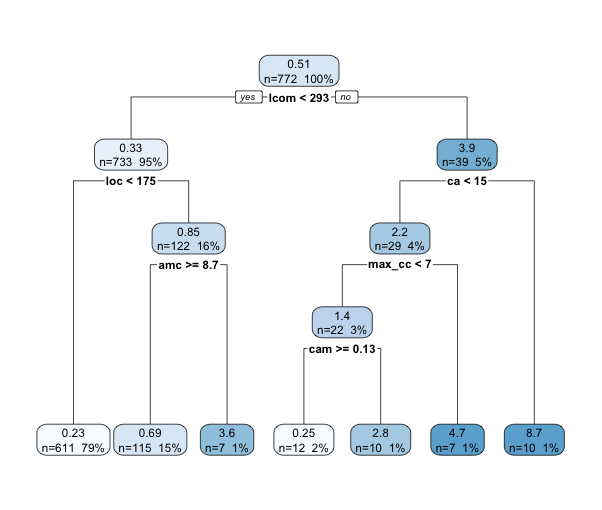
\includegraphics[width=0.72\textwidth]{/Users/rimeljammal/Desktop/Capstone/papers/litreview/images/dtr-ex.png}}
			\caption{An example of a decision tree.}\label{fig:dtr-ex}
		\end{figure}
		\FloatBarrier
		\item Random Forest Regressor (\autoref{fig:rfr-ex}): is an ensemble technique that uses multiple decision trees fitted on different samples from the dataset. The RFR calculates the final prediction based on the average of the predictions of each tree in the ensemble. Creating multiple trees is known to decrease overfitting.
		\begin{figure}[h]
			\centerline{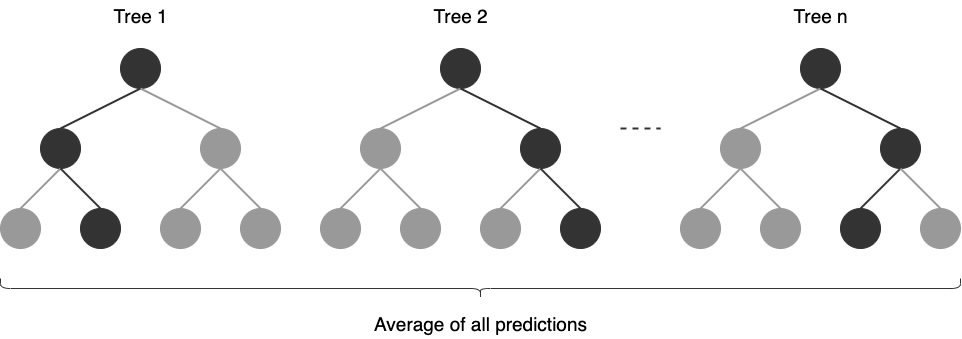
\includegraphics[width=0.9\textwidth]{/Users/rimeljammal/Desktop/Capstone/papers/litreview/images/rfr.png}}
			\caption{An example of a random forest regressor.}\label{fig:rfr-ex}
		\end{figure}
		\item Extra Tree Regressor: same as RFR, but differs in one step which is the way it splits. While RFR takes the local optimal split, ETR takes a random value for the split. It performs well in presence of noisy features and is much faster than RFR.
		\item \textit{k}-Nearest Neighbor Regression: its goal is to find the \textit{k} closest training samples to the new point. In regression tasks, the label of the new point is the mean of the labels of the \textit{k} points nearest neighbors. In the example shown in \autoref{fig:knn-ex}, the new data point will be the mean of the labels of the four nearest points to it.
		\FloatBarrier
		\begin{figure}[h]
			\centerline{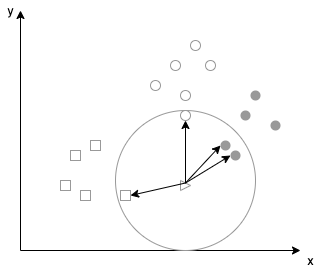
\includegraphics[width=0.4\textwidth]{/Users/rimeljammal/Desktop/Capstone/papers/litreview/images/knn-ex.png}}
			\caption{An example of \textit{k}-NN with \textit{k}=4.}\label{fig:knn-ex}
		\end{figure}
		\FloatBarrier
		\break
		\item Support Vector Regression: invented by \cite{drucker1997support}, follows the same idea as Support Vector Machines (SVM). The goal is to find a function that has at most $\varepsilon$-deviation from the actual label. Where $\varepsilon$ is the accepted margin for errors.
		\FloatBarrier
		\begin{figure}[h]
			\centerline{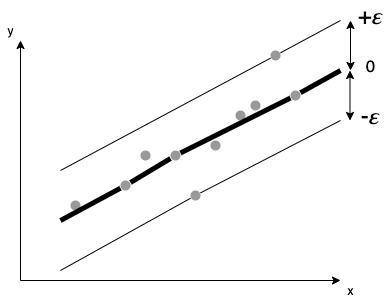
\includegraphics[width=0.5\textwidth]{/Users/rimeljammal/Desktop/Capstone/papers/litreview/images/svr-ex.png}}
			\caption{An example of SVR.}\label{fig:svr-ex}
		\end{figure}
		\FloatBarrier
	\end{itemize}
\break
	\subsection{Stacked Regressor}
	Stacked Regressor is an ensemble learning technique that was first introduced by \cite{wolpert1992stacked}. It consists of multiple base models, and a final model, namely a meta-regressor. The latter predicts the output based on the predictions of the base models.\\
	In our experiments, we implemented two approaches that differ in the meta-regressor used. Both of these approaches consist of the same base models: SVR, ETR, KNN, and DTR. We chose these as base models since they are the most commonly used techniques in this domain.  In the first approach we use SVR as meta-regressor (SR\_SVR) and RFR in the second approach (SR\_RFR). \autoref{fig:sr} shows an illustration of how a SR works.\\
	
	\FloatBarrier
	\begin{figure}[h]
		\centerline{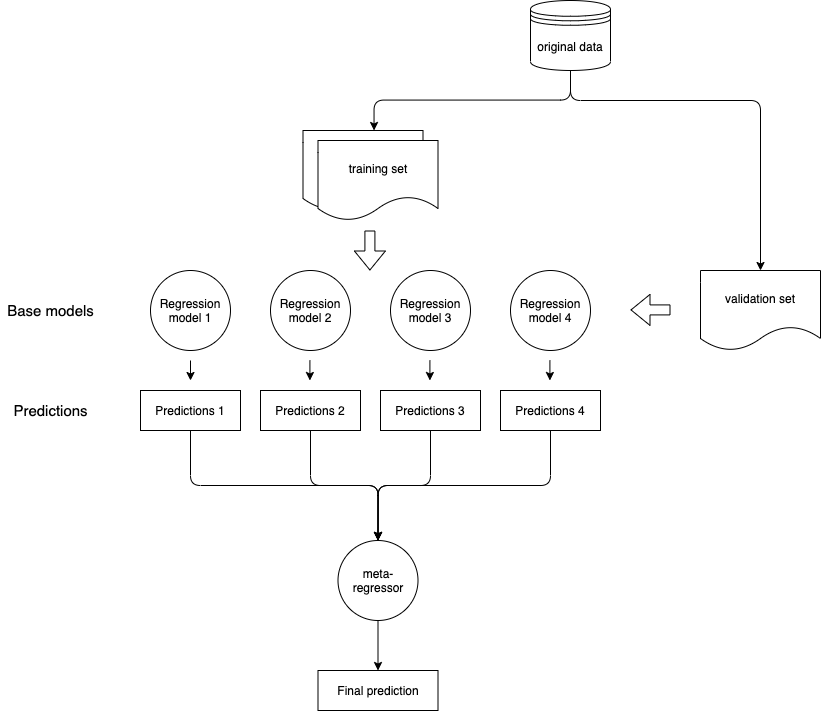
\includegraphics[width=1\textwidth]{/Users/rimeljammal/Desktop/Capstone/papers/litreview/images/sr.png}}
		\caption{Stacked Regressor}\label{fig:sr}
	\end{figure}
	\FloatBarrier
	
	\break
	
	\subsection{Scenarios}
	We conducted experiments on two different scenarios. For each of our experiments, we perform 30 runs and get the average results in each one of them.\\
	Also note that we performed hyperparameter optimization to all of the techniques when running the experiments. 
	\subsubsection{Within-version}
	In this scenario, we keep 20\% of the data aside for validation. We perform 10-fold cross validation on the remaining 80\%. Each time the technique is trained and tested on a fold then validated on the 20\%. We show an illustration of the scenario in \autoref{fig:wv}.
	\FloatBarrier
	\begin{figure}[h]
		\centerline{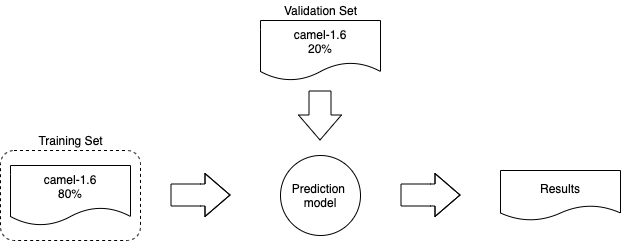
\includegraphics[width=1\textwidth]{/Users/rimeljammal/Desktop/Capstone/papers/litreview/images/wv.png}}
		\caption{Diagram illustrating the within-version scenario.}\label{fig:wv}
	\end{figure}
	\FloatBarrier
	\subsubsection{Within-project}
	In this scenario, we merge all versions of a project except for the last one which we keep as the validation set (\autoref{fig:wp}). Example, in the xalan project, we merge xalan-2.4, xalan-2.5, and xalan-2.6. And use xalan-2.7 as the validation set. Then we perform 10-fold cross validation on the merged set of data (xalan-2.4, xalan-2.5, xalan-2.6) and validate on the last version (xalan-2.7).\\
	
	\FloatBarrier
	\begin{figure}[h]
		\centerline{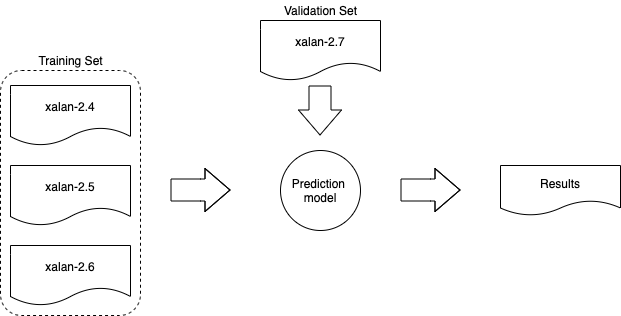
\includegraphics[width=1\textwidth]{/Users/rimeljammal/Desktop/Capstone/papers/litreview/images/wp.png}}
		\caption{Diagram illustrating the within-project scenario.}\label{fig:wp}
	\end{figure}
	\FloatBarrier
	
	\section{Results}
	
	In this section we present the results obtained on the two approaches used. We show the validation results and then the testing results to compare them.
	
	\subsection{Performance Measures}
	We use the following performance measures: mean relative error (MRE), root mean squared error (RMSE), and mean absolute error (MAE). The formulae are shown in \autoref{eq:1}, \autoref{eq:2}, and \autoref{eq:3}. Where \textit{n} is the number of instances, $\overline{y}_{i} $ is the predicted value, and ${y}_{i} $ the actual value.\\
	
	\textbf{RMSE} (\autoref{eq:1}) is used to measure the error between two values, the actual and the predicted number of defects in a particular module. Since the error is squared, this gives importance to big errors. \\
	\begin{equation}
	RMSE = \sqrt{(\frac{1}{n})\sum_{i=1}^{n}(\overline{y}_{i} - y_{i})^{2}} \label{eq:1}
	\end{equation}\break
	\indent \textbf{MAE} (\autoref{eq:2}) is used to measure how far the predicted value is from the actual value. It is the average distance between the actual and predicted errors in the dataset.\\
	\begin{equation}
	MAE = \displaystyle\frac{1}{n}\sum_{i=1}^{n}(|\overline{y}_{i} - y_{i}|) \label{eq:2}
	\end{equation}
	\indent \textbf{MRE} (\autopageref{eq:3}) is used to measure how good a prediction is relatively to the size of the dataset. We have added ``1'' in the denominator to account for the case where ${y}_{i} $ is equal to 0 [\citenum{gao2007comprehensive}], this is when the actual number of defects is 0.\\
		\begin{equation}
		MRE(1) = \displaystyle\frac{1}{n}\sum_{i=1}^{n}(\frac{|y_{i} - \overline{y}_{i}|}{y_{i}+1}) \label{eq:3}
		\end{equation}
	\FloatBarrier
	\subsection{Results and discussion}
	We show both, validation and testing results obtained using the within-version and the within-project scenarios.
	\subsubsection{Within-version}
	Tables (a)-(j) show the validation results obtained on the within-version scenario.
	\begin{itemize}
		\item ant-1.7 (Table (a)): the ant dataset is imbalanced, and the number of defects ranges between 0 and 10. SR\_RFR shows an improvement over all techniques on MRE and MAE. However, ETR obtained the best RMSE among all of the other techniques.
		\item camel-1.6 (Table (b)): this dataset is imbalanced with 80.5\% of the modules being non-defective, and the range of defects between 0 and 28. SR\_RFR outperforms all techniques except SVR who obtained 0.27 as MRE.
	\end{itemize}
	\begin{table}[h]
		\captionsetup[subtable]{labelformat=empty}
		\begin{adjustwidth}{-3.4cm}{}
			\begin{subtable}{9.5cm}
				\centering
				\caption{(a) Validation results on ant-1.7 dataset.}
				\label{tab:ant-wv}
				\begin{tabular}{llll}
					\hline
					ant-1.7 &&&\\ \hline
					Technique & MRE & MAE & RMSE\\  \hline
					DTR & 0.35(0.01) & 0.56(0.01) & 1.24(0.04)\\ 
					RFR & 0.35(0.001) & 0.51(0.001) & 0.93(0.002)\\ 
					ETR & 0.34(0.001) & \bfseries 0.48(0.001) & \bfseries 0.86(0.001)\\ 
					KNN & 0.32(0.004) & \bfseries 0.48(0.005) & 0.88(0.009)\\ 
					SVR & 0.36(0.003) & 0.55(0.005) & 1.005(0.003)\\ 
					SR\_SVR & 0.31(0.02) & 0.48(0.02) & 0.96(0.02)\\
					SR\_RFR & \bfseries 0.27(0.005) & \bfseries 0.47(0.008) & 0.93(0.02)\\ \hline
				\end{tabular}
			\end{subtable}
			\begin{subtable}{9cm}
				\centering
				\caption{(b) Validation results on camel-1.6 dataset.}
				\label{tab:camel-wv}
				\begin{tabular}{llll}
					\hline
					camel-1.6 &&&\\ \hline
					Technique & MRE & MAE & RMSE\\  \hline
					DTR & 0.42(0.01) & 0.81(0.01) & 2.04(0.05)\\ 
					RFR & 0.42(0.001) & 0.8(0.0009) & \bfseries 1.8(0.001)\\ 
					ETR & 0.42(0.0008) & 0.8(0.001) & \bfseries 1.8(0.001)\\ 
					KNN & 0.39(0.004) & 0.79(0.003) & 1.88(0.002)\\ 
					SVR & \bfseries 0.27(0.007) & \bfseries 0.69(0.005) & 1.89(0.002)\\ 
					SR\_SVR & 0.46(0.03) & 0.83(0.02) & \bfseries 1.8(0.01)\\
					SR\_RFR & 0.38(0.01) & 0.89(0.01) & 2.54(0.01)\\ \hline
				\end{tabular}
			\end{subtable} 
		\end{adjustwidth}
	\end{table}
	\FloatBarrier
	\begin{itemize}
		\item ivy-2.0 (Table (c)): on this dataset, the SR\_SVR outperformed all of the other techniques when compared using MRE and MAE by more than 0.06 and 0.04 respectively. However, ETR and RFR scored the lowest RMSE (0.42), whereas SR\_SVR obtained 0.49. In this dataset, the number of defects only ranges between 0 and 3, this explains why the results are more or less better than the ones obtained on other datasets, and it is imbalanced as 88.6\% of the instances have 0 defects.
		\item jedit-4.3 (Table (d)): the errors scored on the jedit dataset were the lowest. We notice that the number of defects in jedit-4.3 ranges only between 0 and 2, and the number of non-defective modules is 97.8\%. TWe believe that the RMSE scored over all of the techniques was low, because there is no big difference between the actual values and the predicted values. 
	\end{itemize}
	\FloatBarrier
	\begin{table}[h]
		\captionsetup[subtable]{labelformat=empty}
		\begin{adjustwidth}{-3.4cm}{}
			\begin{subtable}{9.5cm}
				\centering
				\caption{(c) Validation results on ivy-2.0 dataset.}
				\label{tab:ivy-wv}
				\begin{tabular}{llll}
					\hline
					ivy-2.0 &&&\\ \hline
					Technique & MRE & MAE & RMSE\\  \hline
					DTR & 0.18(0.01) & 0.28(0.01) & 0.66(0.01)\\ 
					RFR & 0.16(0.0006) & 0.24(0.0009) & \bfseries 0.42(0.001)\\ 
					ETR & 0.17(0.0006) & 0.25(0.0008) & \bfseries 0.42(0.0008)\\ 
					KNN & 0.15(0.0005) & 0.23(0.0006) & 0.44(0.001)\\ 
					SVR & 0.24(0.003) & 0.33(0.003) & 0.47(0.002)\\ 
					SR\_SVR & \bfseries 0.09(0.002) & \bfseries 0.19(0.001) & 0.49(0.004)\\
					SR\_RFR & 0.21(0.007) & 0.29(0.006) & 0.51(0.006)\\ \hline
				\end{tabular}
			\end{subtable}
			\begin{subtable}{9cm}
				\centering
				\caption{(d) Validation results on jedit-4.3 dataset.}
				\label{tab:jedit-wv}
				\begin{tabular}{llll}
					\hline
					jedit-4.3 &&&\\ \hline
					Technique & MRE & MAE & RMSE\\  \hline
					DTR & 0.03(0.002) & 0.03(0.002) & 0.18(0.007)\\ 
					RFR & 0.03(0.0003) & 0.04(0.0004) & \bfseries 0.13(0.0002)\\ 
					ETR & 0.03(0.0001) & 0.04(0.0001) & \bfseries 0.13(0.0001)\\ 
					KNN & 0.03(0.0007) & 0.03(0.0007) & 0.14(0.001)\\ 
					SVR & 0.11(0.0004) & 0.12(0.0004) & 0.16(0.0003)\\ 
					SR\_SVR & \bfseries 0.01(0.001) & \bfseries 0.02(0.001) & 0.14(0.001)\\
					SR\_RFR & 0.05(0.005) & 0.07(0.005) & 0.17(0.001)\\ \hline
				\end{tabular}
			\end{subtable} 
		\end{adjustwidth}
	\end{table}
	\begin{itemize}
		\item log4j-1.2 (Table (e)): This dataset is also imbalanced and the majority class is the defective one (92.2\%), and the number of bugs ranges between 0 and 10. SR\_RFR obtained the lowest MAE (0.89) and the lowest RMSE (1.28). Also, SR\_SVR outperformed the other techniques when compared using MRE (0.24). 
		\item lucene-2.4 (Table (f)): the average scored RMSE is relatively high compared to other datasets because the range of the number of defects in this dataset is between 0 and 30. Therefore, the existence of outliers might increase RMSE. Comparing over MRE and MAE, SR\_RFR shows significant improved over MAE, and SR\_SVR obtained the lowest MRE.
	\end{itemize}
	\begin{table}[h]
		\captionsetup[subtable]{labelformat=empty}
		\begin{adjustwidth}{-3.4cm}{}
			\begin{subtable}{9.5cm}
				\centering
				\caption{(e) Validation results on log4j-1.2 dataset.}
				\label{tab:log4j-wv}
				\begin{tabular}{llll}
					\hline
					log4j-1.2 &&&\\ \hline
					Technique & MRE & MAE & RMSE\\  \hline
					DTR & 0.38(0.01) & 1.38(0.04) & 2.15(0.05)\\ 
					RFR & 0.26(0.0007) & 0.91(0.001) & 1.7(0.002)\\ 
					ETR & 0.28(0.001) & 0.94(0.003) & 1.73(0.002)\\ 
					KNN & 0.31(0.001) & 1.08(0.009) & 1.81(0.01)\\ 
					SVR & 0.29(0.0002) & 1.08(0.0005) & 1.86(0.0002)\\ 
					SR\_SVR & \bfseries 0.24(0.005) & 0.97(0.01) & 1.74(0.05)\\
					SR\_RFR & 0.33(0.01) & \bfseries 0.89(0.02) & \bfseries 1.28(0.03)\\ \hline
				\end{tabular}
			\end{subtable}
			\begin{subtable}{9cm}
				\centering
				\caption{(f) Validation results on lucene-2.4 dataset.}
				\label{tab:lucene-wv}
				\begin{tabular}{llll}
					\hline
					lucene-2.4 &&&\\ \hline
					Technique & MRE & MAE & RMSE\\  \hline
					DTR & 0.65(0.02) & 1.96(0.03) & 3.55(0.07)\\ 
					RFR & 0.58(0.003) & 1.7(0.006) & 3.63(0.005)\\
					ETR & 0.57(0.002) & 1.65(0.004) & 3.63(0.0059)\\ 
					KNN & 0.6(0.007) & 1.79(0.01) & 3.45(0.01)\\ 
					SVR & 0.56(0.002) & 1.8(0.003) & 3.84(0.002\\ 
					SR\_SVR & \bfseries 0.52(0.008) & 1.65(0.01) & 3.09(0.05)\\
					SR\_RFR & 0.61(0.01) & \bfseries 1.59(0.01) & \bfseries 2.6(0.04)\\ \hline
				\end{tabular}
			\end{subtable} 
		\end{adjustwidth}
	\end{table}
	\FloatBarrier
	\begin{itemize}
		\item poi-3.0 (Table (g)): the number of defects ranges between 0 and 19. SR\_SVR outperformed all of the techniques when compared using MRE and MAE, and ETR obtained the lowest RMSE (1.15). Here also, we notice a relatively high RMSE due to the large number of class labels (20).
		\item velocity-1.6 (Table (h)): KNN scored the best MRE (0.4), whereas SR\_RFR outperformed the other techniques over MAE (0.92) and RMSE (1.33).
	\end{itemize}
	\FloatBarrier
	\begin{table}[h]
		\captionsetup[subtable]{labelformat=empty}
		\begin{adjustwidth}{-3.4cm}{}
			\begin{subtable}{9.5cm}
				\centering
				\caption{(g) Validation results on poi-3.0 dataset.}
				\label{tab:poi-wv}
				\begin{tabular}{llll}
					\hline
					poi-3.0 &&&\\ \hline
					Technique & MRE & MAE & RMSE\\  \hline
					DTR & 0.48(0.02) & 1.01(0.03) & 2.05(0.08)\\ 
					RFR & 0.44(0.002) & 0.8(0.005) & 1.17(0.005)\\ 
					ETR & 0.41(0.002) & 0.76(0.003) & \bfseries 1.15(0.003)\\ 
					KNN & 0.43(0.0009) & 0.86(0.001) & 1.39(0.003)\\ 
					SVR & 0.44(0.004) & 0.78(0.003) & 1.28(0.002)\\ 
					SR\_SVR & \bfseries 0.39(0.005) & \bfseries 0.72(0.007) & 1.32(0.01)\\
					SR\_RFR & 0.45(0.009) & 0.77(0.01) & 1.23(0.02)\\ \hline
				\end{tabular}
			\end{subtable}
			\begin{subtable}{9cm}
				\centering
				\caption{(h) Validation results on velocity-1.6 dataset.}
				\label{tab:velocity-wv}
				\begin{tabular}{llll}
					\hline
					velocity-1.6 &&&\\ \hline
					Technique & MRE & MAE & RMSE\\  \hline
					DTR & 0.46(0.02) & 1.2(0.04) & 2.41(0.06)\\ 
					RFR & 0.53(0.003) & 1.28(0.003) & 2.38(0.003)\\ 
					ETR & 0.53(0.001) & 1.3(0.002) & 2.44(0.002)\\ 
					KNN & \bfseries 0.4(0.003) & 1.23(0.003) & 2.57(0.004)\\ 
					SVR & 0.52(0.003) & 1.34(0.004) & 2.54(0.002)\\ 
					SR\_SVR & 0.57(0.01) & 1.29(0.01) & 2.38(0.01)\\
					SR\_RFR & 0.63(0.02) & \bfseries 0.92(0.01) & \bfseries 1.33(0.02)\\ \hline
				\end{tabular}
			\end{subtable} 
		\end{adjustwidth}
	\end{table}
	\FloatBarrier
	\begin{itemize}
		\item xalan-2.7 (Table (i)): SR\_SVR outperforms all of the other techniques when compared using MRE and MAE. We notice that xalan-2.7 is imbalanced as 98.8\% of the modules are defective and the number of defects ranges between 0 and 8.
		\item xerces-1.4 (Table (j)): we notice that in this dataset the RMSE is the highest between all of the other datasets. That is because the defect number ranges between 0 and 62, and it contains some outliers. By definition, RMSE gives high importance to big errors. SR\_SVR outperformed the other techniques by scoring the lowest MAE (1.32).
	\end{itemize}
	\FloatBarrier
	\begin{table}[h]
		\captionsetup[subtable]{labelformat=empty}
		\begin{adjustwidth}{-3.4cm}{}
			\begin{subtable}{9.5cm}
				\centering
				\caption{(i) Validation results on xalan-2.7 dataset.}
				\label{tab:xalan-wv}
				\begin{tabular}{llll}
					\hline
					xalan-2.7 &&&\\ \hline
					Technique & MRE & MAE & RMSE\\  \hline
					DTR & 0.14(0.005) & 0.37(0.01) & 0.87(0.03)\\ 
					RFR & 0.13(0.0004) & 0.35(0.0008) & 0.63(0.0009)\\ 
					ETR & 0.13(0.0003) & 0.36(0.0006) & 0.62(0.0007)\\ 
					KNN & 0.12(0.0005) & 0.33(0.001) & 0.67(0.001)\\ 
					SVR & 0.13(0.0003) & 0.33(0.0008) & \bfseries 0.59(0.0006)\\ 
					SR\_SVR & \bfseries 0.11(0.006) & \bfseries 0.31(0.01) & 0.63(0.009)\\
					SR\_RFR & 0.14(0.002) & 0.35(0.004) & 0.69(0.009)\\ \hline
				\end{tabular}
			\end{subtable}
			\begin{subtable}{9cm}
				\centering
				\caption{(j) Validation results on xerces-1.4 dataset.}
				\label{tab:xerces-wv}
				\begin{tabular}{llll}
					\hline
					xerces-1.4 &&&\\ \hline
					Technique & MRE & MAE & RMSE\\  \hline
					DTR & 0.68(0.03) & 1.6(0.04) & 4.05(0.19)\\ 
					RFR & 0.59(0.003) & 1.44(0.005) & 2.89(0.01)\\ 
					ETR & 0.67(0.004) & 1.46(0.006) & \bfseries 2.48(0.01)\\ 
					KNN & 0.66(0.002) & 1.67(0.005) & 3.19(0.01)\\ 
					SVR & 0.55(0.001) & 1.47(0.003) & 2.7(0.002)\\ 
					SR\_SVR & 0.53(0.02) & \bfseries 1.32(0.04) & 2.63(0.04)\\
					SR\_RFR & \bfseries 0.52(0.01) & 1.71(0.03) & 4.1(0.07)\\ \hline
				\end{tabular}
			\end{subtable} 
		\end{adjustwidth}
	\end{table}

Now we show the testing results of the first approach. We report the testing results to compare how far off are they from the validation results.\\
Given the tables below, we notice that the validation and testing results are very similar. In most of the cases, the testing errors are slightly lower than the errors scored in validation.\\
Tables (a')-(j') show the testing results of on the within-version scenario.\\

		\begin{table}[h]
		\captionsetup[subtable]{labelformat=empty}
		\begin{adjustwidth}{-2.9cm}{}
			\begin{subtable}{9cm}
				\centering
				\caption{(a') Testing results on ant-1.7 dataset.}
				\label{tab:ant-wv}
				\begin{tabular}{llll}
					\hline
					ant-1.7 &&&\\ \hline
					Technique & MRE & MAE & RMSE\\  \hline
					DTR & 0.34(0.02) & 0.59(0.03) & 1.26(0.06)\\ 
					RFR & 0.3(0.002) & 0.5(0.003) & 0.92(0.01)\\ 
					ETR & 0.31(0.001) & 0.51(0.002) & 0.92(0.01)\\ 
					KNN & 0.29(0.005) & 0.49(0.007) & 0.94(0.01)\\ 
					SVR & 0.33(0.005) & 0.55(0.007) & 1.01(0.01)\\ 
					SR\_SVR & 0.29(0.02) & 0.51(0.02) & 1.01(0.03)\\
					SR\_RFR & 0.3(0.006) & 0.5(0.009) & 0.93(0.02)\\ \hline
				\end{tabular}
			\end{subtable}
			\begin{subtable}{9cm}
				\centering
				\caption{(b') Testing results on camel-1.6 dataset.}
				\label{tab:camel-wv}
				\begin{tabular}{llll}
					\hline
					camel-1.6 &&&\\ \hline
					Technique & MRE & MAE & RMSE\\  \hline
					DTR & 0.47(0.02) & 0.83(0.03) & 2.04(0.09)\\ 
					RFR & 0.43(0.004) & 0.72(0.005) & 1.51(0.02)\\ 
					ETR & 0.44(0.002) & 0.74(0.002) & 1.5(0.02)\\ 
					KNN & 0.42(0.007) & 0.73(0.008) & 1.59(0.03)\\ 
					SVR & 0.31(0.009) & 0.64(0.008) & 1.55(0.03)\\ 
					SR\_SVR & 0.47(0.03) & 0.77(0.02) & 1.58(0.06)\\
					SR\_RFR & 0.37(0.01) & 0.66(0.01) & 1.41(0.03)\\ \hline
				\end{tabular}
			\end{subtable} 
		\end{adjustwidth}
	\end{table}
	\begin{table}[h]
		\captionsetup[subtable]{labelformat=empty}
		\begin{adjustwidth}{-2.9cm}{}
			\begin{subtable}{9cm}
				\centering
				\caption{(c') Testing results on ivy-2.0 dataset.}
				\label{tab:ivy-wv}
				\begin{tabular}{llll}
					\hline
					ivy-2.0 &&&\\ \hline
					Technique & MRE & MAE & RMSE\\  \hline
					DTR & 0.14(0.02) & 0.21(0.02) & 0.54(0.05)\\ 
					RFR & 0.15(0.002) & 0.22(0.002) & 0.43(0.008)\\ 
					ETR & 0.16(0.0009) & 0.23(0.001) & 0.43(0.008)\\ 
					KNN & 0.14(0.002) & 0.21(0.002) & 0.42(0.007)\\ 
					SVR & 0.24(0.004) & 0.32(0.004) & 0.49(0.008)\\ 
					SR\_SVR & 0.06(0.004) & 0.15(0.003) & 0.44(0.01)\\
					SR\_RFR & 0.16(0.008) & 0.23(0.009) & 0.43(0.01)\\ \hline
				\end{tabular}
			\end{subtable}
			\begin{subtable}{9cm}
				\centering
				\caption{(d') Testing results on jedit-4.3 dataset.}
				\label{tab:jedit-wv}
				\begin{tabular}{llll}
					\hline
					jedit-4.3 &&&\\ \hline
					Technique & MRE & MAE & RMSE\\  \hline
					DTR & 0.03(0.007) & 0.05(0.007) & 0.21(0.02)\\ 
					RFR & 0.03(0.0005) & 0.05(0.0005) & 0.14(0.005)\\ 
					ETR & 0.03(0.0003) & 0.04(0.0004) & 0.14(0.005)\\ 
					KNN & 0.03(0.0009) & 0.04(0.001) & 0.15(0.004)\\ 
					SVR & 0.11(0.0007) & 0.13(0.0007) & 0.18(0.002)\\ 
					SR\_SVR & 0.02(0.002) & 0.04(0.002) & 0.16(0.008)\\
					SR\_RFR & 0.05(0.005) & 0.06(0.005) & 0.14(0.006)\\ \hline
				\end{tabular}
			\end{subtable} 
		\end{adjustwidth}
	\end{table}
	\begin{table}[h]
		\captionsetup[subtable]{labelformat=empty}
		\begin{adjustwidth}{-2.9cm}{}
			\begin{subtable}{9cm}
				\centering
				\caption{(e') Testing results on log4j-1.2 dataset.}
				\label{tab:log4j-wv}
				\begin{tabular}{llll}
					\hline
					log4j-1.2 &&&\\ \hline
					Technique & MRE & MAE & RMSE\\  \hline
					DTR & 0.39(0.03) & 1.12(0.07) & 1.61(0.09)\\ 
					RFR & 0.38(0.003) & 0.95(0.008) & 1.28(0.01)\\ 
					ETR & 0.38(0.003) & 0.92(0.007) & 1.3(0.01)\\ 
					KNN & 0.4(0.007) & 1(0.01) & 1.41(0.02)\\ 
					SVR & 0.41(0.004) & 1.009(0.005) & 1.35(0.01)\\ 
					SR\_SVR & 0.35(0.012) & 0.94(0.03) & 1.35(0.04)\\
					SR\_RFR & 0.35(0.01) & 0.97(0.03) & 1.34(0.03)\\ \hline
				\end{tabular}
			\end{subtable}
			\begin{subtable}{9cm}
				\centering
				\caption{(f') Testing results on lucene-2.4 dataset.}
				\label{tab:lucene-wv}
				\begin{tabular}{llll}
					\hline
					lucene-2.4 &&&\\ \hline
					Technique & MRE & MAE & RMSE\\  \hline
					DTR & 0.71(0.05) & 1.63(0.09) & 2.49(0.15)\\ 
					RFR & 0.77(0.009) & 1.51(0.01) & 2.19(0.02)\\
					ETR & 0.78(0.006) & 1.5(0.009) & 2.17(0.02)\\ 
					KNN & 0.76(0.01) & 1.6(0.02) & 2.29(0.03)\\ 
					SVR & 0.68(0.01) & 1.56(0.01) & 2.38(0.03)\\ 
					SR\_SVR & 0.59(0.02) & 1.31(0.03) & 1.96(0.07)\\
					SR\_RFR & 0.59(0.01) & 1.31(0.03) & 2.09(0.09)\\ \hline
				\end{tabular}
			\end{subtable} 
		\end{adjustwidth}
	\end{table}
	\begin{table}[h]
		\captionsetup[subtable]{labelformat=empty}
		\begin{adjustwidth}{-2.9cm}{}
			\begin{subtable}{9cm}
				\centering
				\caption{(g') Testing results on poi-3.0 dataset.}
				\label{tab:poi-wv}
				\begin{tabular}{llll}
					\hline
					poi-3.0 &&&\\ \hline
					Technique & MRE & MAE & RMSE\\  \hline
					DTR & 0.4(0.04) & 0.88(0.06) & 1.83(0.16)\\ 
					RFR & 0.44(0.005) & 0.9(0.009) & 1.69(0.04)\\ 
					ETR & 0.45(0.003) & 0.9(0.004) & 1.67(0.04)\\ 
					KNN & 0.42(0.0049) & 0.9(0.009) & 1.73(0.04)\\ 
					SVR & 0.42(0.006) & 0.86(0.007) & 1.78(0.05)\\ 
					SR\_SVR & 0.37(0.01) & 0.74(0.01) & 1.57(0.06)\\
					SR\_RFR & 0.4(0.01) & 0.85(0.03) & 1.64(0.08)\\ \hline
				\end{tabular}
			\end{subtable}
			\begin{subtable}{9cm}
				\centering
				\caption{(h') Testing results on velocity-1.6 dataset.}
				\label{tab:velocity-wv}
				\begin{tabular}{llll}
					\hline
					velocity-1.6 &&&\\ \hline
					Technique & MRE & MAE & RMSE\\  \hline
					DTR & 0.47(0.05) & 0.85(0.05) & 1.55(0.07)\\ 
					RFR & 0.518(0.006) & 0.85(0.008) & 1.3(0.02)\\ 
					ETR & 0.53(0.004) & 0.88(0.006) & 1.29(0.02)\\ 
					KNN & 0.46(0.008) & 0.82(0.01) & 1.3(0.02)\\ 
					SVR & 0.53(0.008) & 0.89(0.009) & 1.31(0.03)\\ 
					SR\_SVR & 0.61(0.02) & 0.91(0.02) & 1.32(0.02)\\
					SR\_RFR & 0.49(0.03) & 0.91(0.04) & 1.46(0.07)\\ \hline
				\end{tabular}
			\end{subtable} 
		\end{adjustwidth}
	\end{table}
	\begin{table}[h]
		\captionsetup[subtable]{labelformat=empty}
		\begin{adjustwidth}{-2.9cm}{}
			\begin{subtable}{9cm}
				\centering
				\caption{(i') Testing results on xalan-2.7 dataset.}
				\label{tab:xalan-wv}
				\begin{tabular}{llll}
					\hline
					xalan-2.7 &&&\\ \hline
					Technique & MRE & MAE & RMSE\\  \hline
					DTR & 0.13(0.007) & 0.34(0.01) & 0.8(0.03)\\ 
					RFR & 0.13(0.0009) & 0.33(0.002) & 0.61(0.007)\\ 
					ETR & 0.13(0.0006) & 0.34(0.001) & 0.6(0.005)\\ 
					KNN & 0.11(0.001) & 0.29(0.004) & 0.6(0.01)\\ 
					SVR & 0.14(0.001) & 0.35(0.002) & 0.62(0.007)\\ 
					SR\_SVR & 0.11(0.007) & 0.29(0.01) & 0.62(0.01)\\
					SR\_RFR & 0.12(0.002) & 0.32(0.006) & 0.58(0.01	)\\ \hline
				\end{tabular}
			\end{subtable}
			\begin{subtable}{9cm}
				\centering
				\caption{(j') Testing results on xerces-1.4 dataset.}
				\label{tab:xerces-wv}
				\begin{tabular}{llll}
					\hline
					xerces-1.4 &&&\\ \hline
					Technique & MRE & MAE & RMSE\\  \hline
					DTR & 0.57(0.06) & 2.23(0.15) & 5.2(0.41)\\ 
					RFR & 0.55(0.008) & 1.93(0.02) & 4.06(0.06)\\ 
					ETR & 0.66(0.006) & 2.03(0.01) & 4.03(0.07)\\ 
					KNN & 0.63(0.008) & 2.06(0.02) & 4.18(0.08)\\ 
					SVR & 0.56(0.01) & 2.13(0.02) & 4.68(0.09)\\ 
					SR\_SVR & 0.49(0.03) & 1.9(0.07) & 4.21(0.18)\\
					SR\_RFR & 0.49(0.02) & 1.7(0.05) & 3.64(0.16)\\ \hline
				\end{tabular}
			\end{subtable} 
		\end{adjustwidth}
	\end{table}
	
	\FloatBarrier
	
	\subsubsection{Within-Project results}
	\FloatBarrier
	The results of running the techniques in the within-project scenario on 9 datasets are shown in Tables (k)-(s). The results were obtained on only 9 of the 10 datasets because the ant dataset contains only one version (ant-1.7). 
		\begin{itemize}
		\item camel (Table (k)): the camel dataset when merged is imbalanced (80\% being non-defective), and the number of defects ranges between 0 and 28. SR\_SVR shows an improvement over all techniques on MRE and MAE. However, ETR and RFR obtained the best RMSE among all of the other techniques. In this dataset the validation set consists of 35\% of the data.
		\item ivy (Table (l)): the validation set takes 50\% of this dataset. It is imbalanced with 77\% of the modules being non-defective, and the range of defects between 0 and 36. SR\_SVR outperforms all techniques by more than 0.3 (MRE), and more than 0.28 (MAE).
	\end{itemize}
	\begin{table}[h]
		\captionsetup[subtable]{labelformat=empty}
		\begin{adjustwidth}{-3.4cm}{}
			\begin{subtable}{9.5cm}
				\centering
				\caption{(k) Validation results on the camel dataset.}
				\label{tab:xalan-wv}
				\begin{tabular}{llll}
					\hline
							camel &              &              &              \\ \hline
					Technique & MRE          & MAE          & RMSE         \\ \hline
					DTR       & 0.36(0.008) & 0.68(0.0075) & 1.91(0.0174) \\
					RFR       & 0.45(0.001) & 0.76(0.001) & \bfseries 1.70(0.001) \\
					ETR       & 0.44(0.0004) & 0.76(0.0004) & \bfseries 1.70(0.0008) \\
					KNN       & 0.41(0.0006) & 0.73(0.0006) & 1.75(0.0008) \\
					SVR       & 0.28(0.0005) & 0.62(0.0005) & 1.74(0.0004) \\
					SR\_SVR    & \bfseries 0.22(0.01) & \bfseries 0.59(0.0077) & 1.79(0.02) \\
					SR\_RFR    & 0.33(0.0126) & 0.65(0.0109) & 1.72(0.0078) \\ \hline
				\end{tabular}
			\end{subtable}
			\begin{subtable}{9.5cm}
				\centering
				\caption{(l) Validation results on the ivy dataset.}
				\label{tab:xerces-wv}
				\begin{tabular}{llll}
					\hline
							ivy   &              &              &              \\ \hline
					Technique & MRE          & MAE          & RMSE         \\ \hline
					DTR       & 0.69(0.034 & 0.97(0.04) & 3.58(0.1) \\
					RFR       & 0.59(0.005) & 0.63(0.0054) & 0.90(0.009) \\
					ETR       & 0.60(0.0013) & 0.63(0.0014) & 0.78(0.003) \\
					KNN       & 0.47(0.001) & 0.56(0.0016) & 0.96(0.0065) \\
					SVR       & 0.48(0.005) & 0.53(0.006) & 0.62(0.003) \\
					SR\_SVR    & \bfseries 0.17(0.02) & \bfseries 0.25(0.02) & \bfseries 0.49(0.01) \\
					SR\_RFR    & 0.52(0.07) & 0.63(0.06) & 1.45(0.11) \\ \hline
				\end{tabular}
			\end{subtable} 
		\end{adjustwidth}
	\end{table}
\begin{itemize}
	\item jedit (Table (m)): this dataset is also imbalanced (76\% non-defective modules), and defects range between 0 and 45. 30\% of the dataset is kept as validation and the remaining for training. When comparing over MRE, SR\_SVR outperformed all other techniques (0.58) except for SVR who scored 0.55. 
	\item log4j (Table (n)): the validation set takes 46\% of this dataset. It is imbalanced with 71\% of the modules being non-defective, and the range of defects between 0 and 9. RFR  outperforms STR\_RFR by 0.01 (MRE), and 0.03 (MAE). 
\end{itemize}
	\begin{table}[h]
		\captionsetup[subtable]{labelformat=empty}
		\begin{adjustwidth}{-3.4cm}{}
			\begin{subtable}{9.5cm}
				\centering
				\caption{(m) Validation results on the jedit dataset.}
				\label{tab:xalan-wv}
				\begin{tabular}{llll}
					\hline
						jedit &              &              &              \\ \hline
						Technique & MRE          & MAE          & RMSE         \\ \hline
						DTR       & 0.84(0.03) & 0.89(0.03) & 3.02(0.2) \\
						RFR       & 0.73(0.0029) & 0.76(0.0031) & 1.45(0.01) \\
						ETR       & 0.75(0.0009) & 0.77(0.0011) & 1.34(0.0082) \\
						KNN       & 0.72(0.0015) & 0.74(0.0015) & 1.62(0.01) \\
						SVR       & \bfseries 0.55(0.0029) & \bfseries 0.55(0.002) & \bfseries 0.88(0.01) \\
						SR\_SVR    & 0.58(0.03) & 0.61(0.03) & 1.14(0.05) \\
						SR\_RFR    & 0.62(0.02) & 0.63(0.02) & 1.02(0.11) \\ \hline
				\end{tabular}
			\end{subtable}
			\begin{subtable}{9.5cm}
				\centering
				\caption{(n) Validation results on the log4j dataset.}
				\label{tab:xerces-wv}
				\begin{tabular}{llll}
					\hline
					log4j &              &             &             \\ \hline
					Technique & MRE          & MAE         & RMSE        \\ \hline
					DTR       & 0.55(0.0050) & 1.99(0.014) & 2.45(0.012) \\
					RFR       & \bfseries 0.49(0.0009) & \bfseries 1.81(0.003) & \bfseries 2.26(0.002) \\
					ETR       & 0.50(0.0006) & 1.84(0.001) & \bfseries 2.26(0.002) \\
					KNN       & 0.52(0.0008) & 1.91(0.003) & 2.32(0.002) \\
					SVR       & 0.52(0.0011) & 1.93(0.003) & 2.35(0.002) \\
					SR\_SVR    & 0.51(0.0026) & 1.88(0.011) & 2.31(0.010) \\
					SR\_RFR    & 0.50(0.0048) & 1.84(0.019) & \bfseries 2.26(0.018) \\ \hline
				\end{tabular}
			\end{subtable} 
		\end{adjustwidth}
	\end{table}
	\begin{itemize}
		\item lucene (Table (o)): the validation set consists of 43\% of this dataset and it is balanced since 46\% of the modules are non-defective. The range of defects in this dataset varies between 0 and 47 which allows big errors to occur. This might explain the high RMSE.
		\item poi (Table (p)): the validation set takes 68\% of this dataset. It is also balanced with 54\% of the modules being non-defective, and the range of defects between 0 and 20. STR\_SVR outperforms the other techniques when compared using MRE (0.35). 
	\end{itemize}
	\begin{table}[h]
		\captionsetup[subtable]{labelformat=empty}
		\begin{adjustwidth}{-3.4cm}{}
			\begin{subtable}{9.5cm}
				\centering
				\caption{(o) Validation results on the lucene dataset.}
				\label{tab:xalan-wv}
				\begin{tabular}{llll}
					\hline
					lucene\\ \hline
					Technique & MRE         & MAE         & RSME        \\ \hline
					DTR       & 0.87(0.015) & 2.20(0.026) & 4.45(0.063) \\
					RFR       & 0.68(0.001) & 1.57(0.003) & 2.63(0.003) \\
					ETR       & 0.69(0.002) & \bfseries 1.53(0.003) & 2.59(0.004) \\
					KNN       & 0.63(0.001) & 1.56(0.002) & \bfseries 2.48(0.005) \\
					SVR       & \bfseries 0.56(0.004) & 1.58(0.003) & 2.87(0.002) \\
					SR\_SVR    & 0.70(0.014) & 1.70(0.031) & 2.74(0.095) \\
					SR\_RFR    & 0.72(0.008) & 1.76(0.019) & 2.93(0.067) \\ \hline
				\end{tabular}
			\end{subtable}
			\begin{subtable}{9.5cm}
				\centering
				\caption{(p) Validation results on the poi dataset.}
				\label{tab:xerces-wv}
				\begin{tabular}{llll}
					\hline
					poi   &              &             &              \\ \hline
					Technique & MRE          & MAE         & RMSE         \\ \hline
					DTR       & 0.48(0.0113) & 1.06(0.017) & 1.99(0.032)  \\
					RFR       & 0.36(0.0011) & \bfseries 0.80(0.001) & 1.76(0.002)  \\
					ETR       & 0.37(0.0009) & \bfseries 0.80(0.001) & 1.78(0.004)  \\
					KNN       & 0.39(0.0009) & 0.87(0.001) & 1.79(0.001)  \\
					SVR       & 0.38(0.0022) & 0.90(0.003) & 1.87(0.003)  \\
					SR\_SVR    & \bfseries 0.35(0.0045) & 0.98(0.029) & 2.01(0.050)  \\
					SR\_RFR    & 0.41(0.0067) & 0.85(0.007) & \bfseries 1.71(0.016)  \\ \hline
				\end{tabular}
			\end{subtable} 
		\end{adjustwidth}
	\end{table}
	\begin{itemize}
	\item velocity (Table (q)): the validation set consists of 36\% of this dataset and it is imbalanced since only 29\% of the modules are non-defective. The number of defects ranges between 0 and 10. SR\_SVR outperforms all other techniques by scoring the lowest MRE (0.74), MAE (1.09), and RMSE (1.59).
	\item xalan (Table (r)): the techniques were trained on 72\% of the dataset and validated on the remaining 28\%. The non-defective modules form 62\% of the dataset. RFR, ETR, and KNN outperformed SR\_RFR by 0.01 (MRE), and 0.03 (MAE).
\end{itemize}
		\begin{table}[h]
		\captionsetup[subtable]{labelformat=empty}
		\begin{adjustwidth}{-3.4cm}{}
			\begin{subtable}{9.5cm}
				\centering
				\caption{(q) Validation results on the velocity dataset.}
				\label{tab:xalan-wv}
				\begin{tabular}{llll}
					\hline
					velocity &             &              &             \\ \hline
					Technique    & MRE         & MAE          & RMSE        \\ \hline
					DTR          & 0.76(0.008) & 1.16(0.01) & 1.84(0.026) \\
					RFR          & 0.86(0.001) & 1.21(0.001) & 1.66(0.001) \\
					ETR          & 0.87(0.001) & 1.22(0.001) & 1.67(0.001) \\
					KNN          & 0.84(0.001) & 1.22(0.001) & 1.71(0.002) \\
					SVR          & 0.81(0.004) & 1.18(0.0061) & 1.72(0.007) \\
					SR\_SVR       & \bfseries 0.74(0.008) & \bfseries 1.09(0.009) & \bfseries 1.59(0.01) \\
					SR\_RFR       & 0.77(0.020) & 1.12(0.0215) & 1.66(0.020) \\ \hline
				\end{tabular}
			\end{subtable}
			\begin{subtable}{9.5cm}
				\centering
				\caption{(r) Validation results on the xalan dataset.}
				\label{tab:xerces-wv}
				\begin{tabular}{llll}
					\hline
					xalan &              &              &              \\ \hline
					Technique & MRE          & MAE          & RMSE         \\ \hline
					DTR       & 0.39(0.004) & 0.92(0.01) & 1.17(0.01) \\
					RFR       & \bfseries 0.32(0.0003) & 0.80(0.0009) & 0.99(0.0008) \\
					ETR       & \bfseries 0.32(0.0002) & \bfseries 0.79(0.0007) & \bfseries 0.98(0.0009) \\
					KNN       & \bfseries 0.32(0.0003) & \bfseries 0.79(0.0006) & 1.00(0.0007) \\
					SVR       & 0.36(0.0002) & 0.88(0.0005) & 1.09(0.0004) \\
					SR\_SVR    & 0.37(0.009) & 0.92(0.02) & 1.11(0.02) \\
					SR\_RFR    & 0.33(0.004) & 0.82(0.0092) & 1.04(0.008) \\ \hline
				\end{tabular}
			\end{subtable} 
		\end{adjustwidth}
	\end{table}
\FloatBarrier
	\begin{itemize}
	\item xerces (Table (s)): training was done on 64\% of this dataset. We also notice that it is imbalanced since only 20\% of the modules are defective. The number of defects ranges between 0 and 30. When comparing using MRE, SR\_ outperforms all techniques (0.48) expect for SVR (0.46).
\end{itemize}
\FloatBarrier
		\begin{table}[h]
	\captionsetup[subtable]{labelformat=empty}
	\begin{adjustwidth}{1.5cm}{}
		\begin{subtable}{9cm}
			\centering
			\caption{(s) Validation results on the xerces dataset.}
			\label{tab:xalan-wv}
			\begin{tabular}{llll}
				\hline
				xerces &              &              &              \\ \hline
				Technique  & MRE          & MAE          & RMSE    \\ \hline
				DTR        & 0.53(0.002) & 2.54(0.01) & \bfseries 5.34(0.03)  \\
				RFR        & 0.53(0.0008) & 2.55(0.0022) & 5.51(0.003) \\
				ETR        & 0.50(0.0008) & \bfseries 2.51(0.0017) & 5.53(0.004) \\
				KNN        & 0.51(0.0008) & 2.58(0.0009) & 5.68(0.0007) \\
				SVR        & \bfseries 0.46(0.001) & \bfseries 2.51(0.0020) & 5.68(0.0028)  \\
				SR\_SVR     & 0.48(0.0025) & 2.59(0.01) & 5.69(0.01)  \\
				SR\_RFR     & 0.50(0.0018) & \bfseries 2.51(0.0082) & 5.54(0.01) \\ \hline
			\end{tabular}
		\end{subtable}
	\end{adjustwidth}
\end{table}
\break
\FloatBarrier
Tables (k')-(s') show the testing results on the within-project scenario. No significant difference was reported between the validation and the testing results.\\
\FloatBarrier
\FloatBarrier
	\begin{table}[h]
	\captionsetup[subtable]{labelformat=empty}
	\begin{adjustwidth}{-3.4cm}{}
		\begin{subtable}{9.5cm}
			\centering
			\caption{(k') Testing results on the camel dataset.}
			\label{tab:xalan-wv}
			\begin{tabular}{llll}
				\hline
				camel &              &              &              \\ \hline
				Technique & MRE          & MAE          & RMSE         \\ \hline
				DTR       & 0.39(0.0195) & 0.67(0.0202) & 1.65(0.0598) \\
				RFR       & 0.42(0.0025) & 0.68(0.0028) & 1.29(0.0128) \\
				ETR       & 0.43(0.0011) & 0.69(0.0013) & 1.29(0.0113) \\
				KNN       & 0.39(0.0030) & 0.67(0.0033) & 1.34(0.0126) \\
				SVR       & 0.27(0.0033) & 0.57(0.0042) & 1.34(0.0149) \\
				SR\_SVR    & 0.22(0.0144) & 0.54(0.0081) & 1.36(0.0285) \\
				SR\_RFR    & 0.34(0.0157) & 0.61(0.0138) & 1.31(0.0401) \\ \hline
			\end{tabular}
		\end{subtable}
		\begin{subtable}{9.5cm}
			\centering
			\caption{(l') Testing results on the ivy dataset.}
			\label{tab:xerces-wv}
			\begin{tabular}{llll}
				\hline
				ivy   &              &              &              \\ \hline
				Technique & MRE          & MAE          & RMSE         \\ \hline
				DTR       & 0.69(0.0706) & 1.27(0.0786) & 3.38(0.3023) \\
				RFR       & 0.57(0.0080) & 1.00(0.0099) & 2.09(0.0612) \\
				ETR       & 0.58(0.0047) & 1.01(0.0052) & 2.06(0.0681) \\
				KNN       & 0.49(0.0098) & 0.94(0.0120) & 2.12(0.0634) \\
				SVR       & 0.51(0.0054) & 0.99(0.0052) & 2.11(0.0878) \\
				SR\_SVR    & 0.23(0.0209) & 0.78(0.0162) & 2.15(0.0931) \\
				SR\_RFR    & 0.55(0.0675) & 1.07(0.0585) & 2.58(0.1394) \\ \hline
			\end{tabular}
		\end{subtable} 
	\end{adjustwidth}
\end{table}

\begin{table}[h]
	\captionsetup[subtable]{labelformat=empty}
	\begin{adjustwidth}{-3.4cm}{}
		\begin{subtable}{9.5cm}
			\centering
			\caption{(m') Testing results on the jedit dataset.}
			\label{tab:xalan-wv}
			\begin{tabular}{llll}
				\hline
				jedit &              &              &              \\ \hline
				Technique & MRE          & MAE          & RMSE         \\ \hline
				DTR       & 0.42(0.0249) & 0.91(0.0338) & 2.52(0.1529) \\
				RFR       & 0.45(0.0038) & 0.84(0.0055) & 1.98(0.0267) \\
				ETR       & 0.45(0.0029) & 0.83(0.0055) & 1.91(0.0258) \\
				KNN       & 0.45(0.0050) & 0.85(0.0068) & 1.99(0.0325) \\
				SVR       & 0.37(0.0100) & 0.84(0.0113) & 2.20(0.0441) \\
				SR\_SVR    & 0.35(0.0218) & 0.75(0.0254) & 1.88(0.0539) \\
				SR\_RFR    & 0.39(0.0140) & 0.81(0.0244) & 2.04(0.0885) \\ \hline
			\end{tabular}
		\end{subtable}
		\begin{subtable}{9.5cm}
			\centering
			\caption{(n') Testing results on the log4j dataset.}
			\label{tab:xerces-wv}
			\begin{tabular}{llll}
				\hline
				log4j &             &             &            \\ \hline
				Technique & MRE         & MAE         & RMSE       \\ \hline
				DTR       & 0.34(0.026) & 0.63(0.044) & 1.21(0.06) \\
				RFR       & 0.36(0.005) & 0.62(0.007) & 1.01(0.01) \\
				ETR       & 0.38(0.003) & 0.63(0.004) & 1.00(0.01) \\
				KNN       & 0.30(0.009) & 0.57(0.015) & 1.01(0.02) \\
				SVR       & 0.30(0.014) & 0.60(0.017) & 1.09(0.02) \\
				SR\_SVR    & 0.32(0.011) & 0.59(0.019) & 1.03(0.04) \\
				SR\_RFR    & 0.33(0.016) & 0.59(0.022) & 1.05(0.05) \\ \hline
			\end{tabular}
		\end{subtable} 
	\end{adjustwidth}
\end{table}

\begin{table}[h]
	\captionsetup[subtable]{labelformat=empty}
	\begin{adjustwidth}{-3.4cm}{}
		\begin{subtable}{9.5cm}
			\centering
			\caption{(o') Testing results on the lucene dataset.}
			\label{tab:xalan-wv}
			\begin{tabular}{llll}
				\hline
				lucene &             &             &             \\ \hline
				Technique  & MRE         & MAE         & RMSE        \\ \hline
				DTR        & 0.62(0.032) & 1.41(0.060) & 2.53(0.158) \\
				RFR        & 0.68(0.006) & 1.40(0.011) & 2.46(0.036) \\
				ETR        & 0.70(0.004) & 1.39(0.007) & 2.43(0.038) \\
				KNN        & 0.64(0.008) & 1.39(0.015) & 2.51(0.047) \\
				SVR        & 0.59(0.011) & 1.47(0.016) & 2.76(0.046) \\
				SR\_SVR     & 0.56(0.01)  & 1.26(0.029) & 2.27(0.084) \\
				SR\_RFR     & 0.57(0.01)  & 1.28(0.031) & 2.32(0.103) \\ \hline
			\end{tabular}
		\end{subtable}
		\begin{subtable}{9.5cm}
			\centering
			\caption{(p') Testing results on the poi dataset.}
			\label{tab:xerces-wv}
			\begin{tabular}{llll}
				\hline
				poi   &              &             &              \\ \hline
				Technique & MRE          & MAE         & RMSE         \\ \hline
				DTR       & 0.65(0.018)  & 1.16(0.030) & 1.91(0.0908) \\
				RFR       & 0.56(0.002)  & 0.94(0.003) & 1.47(0.013)  \\
				ETR       & 0.57(0.001)  & 0.94(0.002) & 1.47(0.013)  \\
				KNN       & 0.56(0.004)  & 0.98(0.006) & 1.55(0.0168) \\
				SVR       & 0.58(0.009)  & 1.06(0.012) & 1.69(0.0166) \\
				SR\_SVR    & 0.39(0.028)  & 0.95(0.015) & 1.67(0.031)  \\
				SR\_RFR    & 0.64(0.009)  & 1.11(0.013) & 1.70(0.023)  \\ \hline
			\end{tabular}
		\end{subtable} 
	\end{adjustwidth}
\end{table}

\begin{table}[h]
	\captionsetup[subtable]{labelformat=empty}
	\begin{adjustwidth}{-3.4cm}{}
		\begin{subtable}{9.5cm}
			\centering
			\caption{(q') Testing results on the velocity dataset.}
			\label{tab:xalan-wv}
			\begin{tabular}{llll}
				\hline
				velocity &             &              &             \\ \hline
				Technique    & MRE         & MAE          & RMSE        \\ \hline
				DTR          & 0.49(0.032) & 1.03(0.048)  & 1.72(0.087) \\
				RFR          & 0.49(0.004) & 0.90(0.008)  & 1.33(0.014) \\
				ETR          & 0.48(0.001) & 0.89(0.003)  & 1.32(0.010) \\
				KNN          & 0.52(0.004) & 0.98(0.007)  & 1.42(0.012) \\
				SVR          & 0.54(0.010) & 1.02(0.015)  & 1.47(0.021) \\
				SR\_SVR       & 0.44(0.011) & 0.87(0.018)  & 1.37(0.026) \\
				SR\_RFR       & 0.55(0.020) & 0.99(0.024)  & 1.48(0.035) \\ \hline
			\end{tabular}
		\end{subtable}
		\begin{subtable}{9.5cm}
			\centering
			\caption{(r') Testing results on the xalan dataset.}
			\label{tab:xerces-wv}
			\begin{tabular}{llll}
				\hline
				xalan &              &              &              \\ \hline
				Technique & MRE          & MAE          & RMSE         \\ \hline
				DTR       & 0.38(0.0065) & 0.59(0.0085) & 1.00(0.0194) \\
				RFR       & 0.36(0.0008) & 0.54(0.0013) & 0.77(0.0030) \\
				ETR       & 0.36(0.0005) & 0.55(0.0008) & 0.77(0.0029) \\
				KNN       & 0.35(0.0016) & 0.54(0.0021) & 0.80(0.0039) \\
				SVR       & 0.32(0.0035) & 0.53(0.0038) & 0.88(0.0054) \\
				SR\_SVR    & 0.31(0.0111) & 0.52(0.0081) & 0.82(0.0143) \\
				SR\_RFR    & 0.37(0.0055) & 0.56(0.0055) & 0.87(0.0101) \\ \hline
			\end{tabular}
		\end{subtable} 
	\end{adjustwidth}
\end{table}

\begin{table}[h]
	\captionsetup[subtable]{labelformat=empty}
	\begin{adjustwidth}{1.5cm}{}
		\begin{subtable}{9cm}
			\centering
			\caption{(s') Testing results on the xerces dataset.}
			\label{tab:xalan-wv}
			\begin{tabular}{llll}
				\hline
				xerces &              &              &              \\ \hline
				Technique  & MRE          & MAE          & RMSE    \\ \hline
				DTR        & 0.31(0.0117) & 0.57(0.0174) & 1.41(0.0664)  \\
				RFR        & 0.38(0.0035) & 0.62(0.0042) & 1.22(0.0176) \\
				ETR        & 0.39(0.0018) & 0.63(0.0027) & 1.21(0.0201)  \\
				KNN        & 0.34(0.0024) & 0.59(0.0035) & 1.22(0.0187)   \\
				SVR        & 0.33(0.0048) & 0.58(0.0062) & 1.29(0.0212) \\
				SR\_SVR     & 0.24(0.0127) & 0.51(0.0101) & 1.25(0.0289) \\
				SR\_RFR     & 0.32(0.0057) & 0.55(0.0082) & 1.24(0.0267) \\ \hline
			\end{tabular}
		\end{subtable}
	\end{adjustwidth}
\end{table}
\FloatBarrier
\section{Threats to internal validity}
We used the most common and widely used datasets. They are publicly available on this URL: \href{https://zenodo.org/communities/seacraft/search?page=1&size=20&keywords=defect#}{seacraft repository}. They are based on the CK metrics proposed by \cite{chidamber1994metrics}. These might not be the only features affecting the results, and are not the only metrics used in the literature. However, they are widely used in this domain.
\section{Threats to external validity}
We tested the proposed technique on a specific dataset, which can't be generalized to all other software modules used in the industry. We experimented on multiple scenarios and on balanced and imbalanced datasets with different sizes to see how the techniques would perform. Also, we ran experiments by training on different projects having various ranges of defects.\\
We did not test Stacked Regressors on different metrics since all of the datasets we used share the same features. It would be interesting to see the results when applied on different metrics.\\
Another interesting thing to try is predicting if the module is defective or not. In the case where developers are not interested in the number of defects in a module, it would be interesting to test the proposed techniques on classification.
\section{Conclusion}
In our work, we proposed using a new regression technique to predict the number of defects in a software module. This technique is called Stacked Regressor and is an ensemble model. But instead of averaging the prediction of the base models, they are passed to another regressor that does the final prediction. We used two approaches for this technique, by changing the final predictor. In the first one we use SVR, and in the second one we use RFR. Then we compared this technique to five other regression models. Results of the Stacked Regressor show to be promising as the two different approaches outperform the other techniques on most of the datasets.\\
Furthermore optimization could be done to the Stacked Regressor by trying different combinations of models or by applying PCA to the meta-features, i.e. reduce the number of features when passed to the Stacked Regressor.
\FloatBarrier
\break
\bibliography{ref}{}
\bibliographystyle{apalike}
	
\end{document}
